\documentclass{article}      % Specifies the document class

% -------------------- Packages --------------------
\usepackage{amsmath}
\usepackage{amssymb}
\usepackage[noend]{algpseudocode}
\usepackage{algorithm}
\usepackage{graphicx}
\usepackage{float}
\usepackage{fontawesome5}
\usepackage{listings}

\lstset{language=Python,keywordstyle={\bfseries \color{blue}}}
\NewDocumentCommand{\codeword}{v}{%
    \texttt{\textcolor[HTML]{5c5c65}{#1}}%
}


\usepackage{hyperref}
\hypersetup{
    colorlinks=true,
    linkcolor=blue,
    filecolor=magenta,      
    urlcolor=cyan,
    pdftitle={Rapport Probabilités et statistiques},
    pdfpagemode=FullScreen,
    }

\urlstyle{same}

\usepackage{bookmark}
\hypersetup{hidelinks} %enlève les cadres rouges autour des hyperliens


% ---------- PSEUDO CODE : hack to remove indent ----------
% https://tex.stackexchange.com/questions/354564/how-to-remove-leading-indentation-from-algorithm
\usepackage{xpatch}
\makeatletter
\xpatchcmd{\algorithmic}
  {\ALG@tlm\z@}{\leftmargin\z@\ALG@tlm\z@}
  {}{}
\makeatother

\usepackage{xcolor}
\usepackage[framemethod=tikz]{mdframed}
\usepackage{tikzpagenodes}
\usetikzlibrary{calc}

% add foreach
\algnewcommand\algorithmicforeach{\textbf{for each}}
\algdef{S}[FOR]{ForEach}[1]{\algorithmicforeach\ #1\ \algorithmicdo}



% -------------------- Couleurs --------------------
\definecolor{definition}{HTML}{2f80ed}
\definecolor{definition-bg}{HTML}{e0ecfd}

\definecolor{danger}{HTML}{e6505f}
\definecolor{danger-bg}{HTML}{fce5e7}

\definecolor{exogris}{gray}{0.4}



% -------------------- Code --------------------
\definecolor{codegreen}{rgb}{0,0.6,0}
\definecolor{codegray}{rgb}{0.5,0.5,0.5}
\definecolor{codepurple}{rgb}{0.58,0,0.82}
\definecolor{backcolour}{rgb}{0.95,0.95,0.92}

\lstdefinestyle{code-style}{
    backgroundcolor=\color{backcolour},   
    commentstyle=\color{codegreen},
    keywordstyle=\color{magenta},
    numberstyle=\tiny\color{codegray},
    stringstyle=\color{codepurple},
    basicstyle=\ttfamily\footnotesize,
    breakatwhitespace=false,         
    breaklines=true,                 
    captionpos=b,                    
    keepspaces=true,                 
    numbers=left,                    
    numbersep=5pt,
    showspaces=false,                
    showstringspaces=false,
    showtabs=false,                  
    tabsize=2
}

% -------------------- Styles --------------------
\mdfdefinestyle{definition-style}{%
  innertopmargin=10px,
  innerbottommargin=10px,
  linecolor=definition,
  backgroundcolor=definition-bg,
  roundcorner=4px
}
\newmdenv[style=definition-style]{definition}

\mdfdefinestyle{danger-style}{%
  innertopmargin=10px,
  innerbottommargin=10px,
  linecolor=danger,
  backgroundcolor=danger-bg,
  roundcorner=4px
}
\newmdenv[style=danger-style]{danger}


% -------------------- Document --------------------
\title{Probabilités et Statistiques\\\Large{Projet noté}}
\author{MADANI Abdenour\\TRIOLET Hugo}
\date{Licence 3\\2021 - 2022}
\begin{document}
\normalsize
\maketitle

\renewcommand*\contentsname{Table des matières}
\tableofcontents
\newpage



\section{Introduction}
\subsection{Objectifs}
Les objectifs de ce TPs sont :
\begin{itemize}
  \item implémenter nous-mêmes plusieurs algorithmes de régression linéaire et les comparer à des fonctions issues de librairies scientifiques
  \item manipuler différentes lois vues en cours via leur implémentation issues de librairies scientifiques
  \item déterminer des intervalles de confiance et effectuer des applications sur quelques exemples
\end{itemize}

On utilisera pour ceci \textbf{Python} et les bibliothèques de fonctions : Numpy, Scipy, Matplotlib, et Statsmodels, entre autres.



\subsection{Définitions}

Hugo : tu peux virer ça si t'as aucune définition à mettre
(tu peux la réutiliser plus bas et virer cette partie aussi)
\begin{definition}
{ \scriptsize \textcolor{definition}{\faIcon{graduation-cap} \textbf{DÉFINITION}}}
\vspace{3px}
\\ \underline{\textbf{Mot défini}}
\vspace{2.5px}
\\ Définition ici
\end{definition}


\subsection{Résumé de notre approche}
Nous avons 3 fichiers, 1 pour chaque TP.
\\%
\\Vis-à-vis du code, nous l’avons documenté à l’aide de la docstring de Python, ainsi que des commentaires normaux : les fonctions se comprennent donc naturellement grâce à ceux-ci.

\section{Régression linéaire}
\subsection{Régression Linéaire simple}
La fonction calculant la régression linéaire simple est "regression\_lineaire".
\\%
\\Étant donné deux listes $x$ et $y$ de même taille, elle calcule la régression linéaire $$y = \beta_1 \cdot x + \beta_0$$
%

\subsubsection{Modèle vectoriel}
On applique simplement la formule donnée dans le TP.

La fonction calculant la régression linéaire simple est "regression\_lineaire\_vec".
\\%
\\Étant donné deux listes $x$ et $y$ de même taille, elle calcule la régression linéaire en utilisant la méthode vectorielle : $$y = \beta_1 \cdot x + \beta_0$$
%


\subsubsection{Résultats obtenus}
\begin{figure}[H]
    \centering
     \scalebox{.5}{
        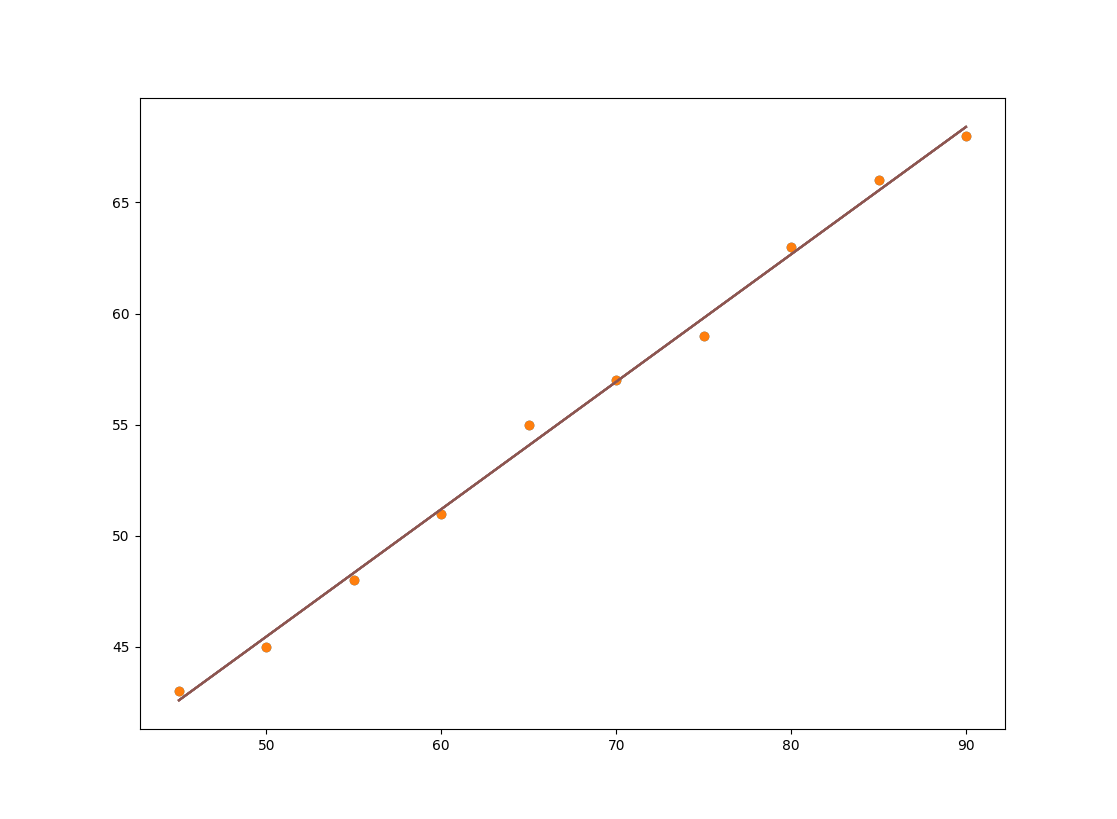
\includegraphics{img/reglin.png}
    }
    \\Représentation graphique obtenue avec Matplotlib
\end{figure}
%
En orange sont affichés les points de $(x_i, y_i)$, et on voit plusieurs droites superposées de couleurs différentes, quasiment indiscernables : ce sont nos deux régressions linéaires ainsi que celle de Numpy (polyfit).
\\Les résultats sont donc concordants : visuellement, toutes les régressions linéaires donnent le même résultat sur ce jeu de donnée.
%
\\Les coeffcients sont de mêmes très proches voire égaux.

\subsection{Régression linéaire et descente de gradient}
Hugo : todo

\section{Étude et manipulation de lois de probabilités}
\subsection{Loi Binomiale}
texte

Si tu veux mettre une image Hugo
\begin{figure}[H]
    \centering
     \scalebox{.35}{  % le chiffre c'est le pourcentage à laquelle l'image est scale
                      % ici c'est 0.35 donc 35%
        %\includegraphics{adresse-image.png}
    }
\end{figure}

\subsection{Loi Normale univariée}
texte
\subsection{Simulation de données à partir d’une loi}
texte

\subsubsection{Cas de la loi normale}
texte

\subsection{Estimation de densité}
texte

\subsubsection{Cas de la loi normale}
texte
\subsubsection{Cas de la loi exponentielle}
texte


\section{Intervalles de confiance}
Le but de cette partie (correspondant au fichier \textsl{tp_3.py}) est de déterminer les intervalles de confiances de différents échantillons statistiques afin de situer, selon une certaine précision, dans quelle plage de valeurs se situe l'espérance de l'échantillon.\\
Dans les 2 premiers problèmes, nous ne connaissons pas la variance de l'échantillon, ainsi la fonction calculant l'intervalle de confiance des échantillons utilisera la méthode de calcul via l'écart-type empirique et le fractile \textit{t} d'ordre 1 - \dfrac{\alpha}{2} de la loi de student \mathit{St(n-1). Le problème 3, quant à lui, modélise un échantillon de taille \mathit{n} de \mathit{B(p = \dfrac{1}{2})}. Ainsi la variance de la loi de Bernoulli est connue et vaut \mathit{p(1-p)}, donc dans ce cas-là, le calcul de l'intervalle de confiance se fera via la formule utilisant l'écart-type véritable et \textit{u} le fractile d'ordre 1 - \dfrac{\alpha}{2} de la loi \mathit{N(0,1)}.

\subsection{Fonctions}

\subsection{Problème 1}
On possède deux échantillons de taille 16 à notre disposition : un échantillon de masses de 16 pots de confitures mesurée en kilogramme (kg), et l'autre de masses d'avocats provenant du Mexique mesurée en grammes (g).\\
\subsection{Problème 2}
texte
\subsection{Problème 3}
texte



\section{Exemples d'utilisation du code}
\subsection{Comment utiliser le code}
Concernant le code, il est séparé en trois fichier, chacun correspondant par son indice à la partie du TP correspondante (\textsl{tp_3.py} avec la partie 3, \textsl{TP2.py} avec la partie 2, ...).
Si le code est exécuté sur l'IDE \texttt{Pyzo}, alors il est possible (après avoir exécuté "l'en-tête" du code, c'est à dire de la première ligne  au premier ##) d'exécuter séparément chaque sous partie du code, délimitées par \textit{## Problème x}.\\
Autrement, le code s'exécute normalement et en entier, si \texttt{Pyzo} n'est pas le logiciel où celui-ci est exécuté.


\end{document}
